\SourcePage{GELFAND-P000456}{unlabelled}
\underline{The seminar will start at \mbox{$18^{\underline{00}}$}.}

\uuline{2/X-72.}\qquad \underline{A. Gabrielov.}

$S$ — compl. analytic set

$H_{\mathbb Z}$ — loc. free $\mathbb Z$-sheaf

($\mathbb Z$ — const. sheaf; a section over a conn. region is a const. integer;
$H_{\mathbb Z}$ — loc. free sheaf of $\mathbb Z$-modules.
\Unclear{GELFAND-P000456}{modules-old}{Overlapping strokes follow “modules.” Their reading is uncertain.}
\end{GelfandAdjacentEvidence}
\begin{GelfandAdjacentEvidence}{GELFAND-P000456}{2}

At $\forall$ point $\exists$ nbhd.,
in which it is isom. to $\mathbb Z\oplus\cdots\oplus\mathbb Z$).

\sout{\mbox{$H$}\ldots}\quad
\Unclear{GELFAND-P000456}{start-old-fragment}{The first crossed-out sign provisionally reads $H$.}
\end{GelfandAdjacentEvidence}
\begin{GelfandAdjacentEvidence}{GELFAND-P000456}{3}

\Incomplete{GELFAND-P000456}{start-cancelled}{The rest of the short entry before the parenthesis is illegible.}
\end{GelfandAdjacentEvidence}
\begin{GelfandAdjacentEvidence}{GELFAND-P000456}{4}

($\mathbb Z$-sheaf assoc. with the presheaf which \sout{\ldots}\ \sout{\ldots}
\par\noindent\hspace*{2em}$F(U)=\mathbb Z$).
\Incomplete{GELFAND-P000456}{presheaf-full-cancel}{Two entries after “which” are crossed out. Below them is $F(U)=\mathbb Z$.}
\end{GelfandAdjacentEvidence}
\begin{GelfandAdjacentEvidence}{GELFAND-P000456}{5}


The space is loc. connected $\Rightarrow$ fiber $=\mathbb Z$.

The space of the sheaf $\mathbb Z$ is homeom. to $S\times\mathbb Z$.

Loc. $\left.H_{\mathbb Z}\right|_U\simeq U\times\mathbb Z^n$
\[
\Gamma(U,H_{\mathbb Z})\cong\mathbb Z^n
\]
$S$ is connected $\Rightarrow$ $n$ is the same everywhere.

Cover by neighborhoods and fix isomorphisms over the neighborhoods\\
\hspace*{2em}(up to $GL(n,\mathbb Z)$)

\SourceFigure{GELFAND-P000456}{overlap-sketch}{Two overlapping ovals with four strokes in their intersection. There is an angular mark on the left arc.
\par\smallskip\centering\color{black}
\begingroup\color{black}\GelfandFitDiagram{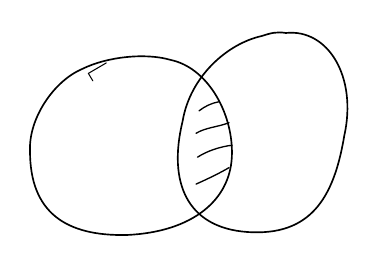
\begin{tikzpicture}[x=.19mm,y=-.19mm,line cap=round,line join=round]
\draw[line width=.6pt] (54,35)
  .. controls (35,43) and (18,68) .. (19,90)
  .. controls (19,131) and (43,147) .. (84,146)
  .. controls (127,144) and (154,123) .. (154,91)
  .. controls (154,63) and (137,34) .. (113,29)
  .. controls (96,24) and (70,27) .. (54,35);
\draw[line width=.6pt] (174,13)
  .. controls (151,18) and (126,40) .. (121,70)
  .. controls (111,111) and (124,141) .. (164,144)
  .. controls (206,147) and (222,122) .. (229,80)
  .. controls (238,40) and (218,8) .. (190,11)
  .. controls (184,10) and (180,11) .. (174,13);
\draw[line width=.38pt] (70,31)--(58,38)--(61,43);
\draw[line width=.48pt]
 (132,63)..controls(136,60)and(140,58)..(145,57)
 (130,78)..controls(137,74)and(144,74)..(152,71)
 (131,94)..controls(137,90)and(146,87)..(154,86)
 (130,112)..controls(139,108)and(147,104)..(152,101);
\end{tikzpicture}}\endgroup}
\end{GelfandAdjacentEvidence}
\begin{GelfandAdjacentEvidence}{GELFAND-P000456}{6}


transition functions from $GL(n,\mathbb Z)$.

One can construct a \uwave{loc. triv.} bundle with such transition functions.

\SourceFigure{GELFAND-P000456}{complex-bundle-link}{A slanted stroke links $H_{\mathbb C}$ to the caption.
\par\smallskip\centering\color{black}
\begingroup\color{black}\GelfandFitDiagram{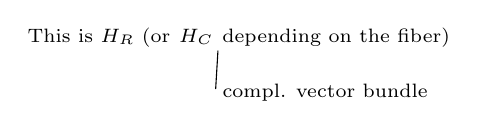
\begin{tikzpicture}[x=1mm,y=1mm,line cap=round,every node/.style={inner sep=0pt,anchor=base west,font=\scriptsize}]
\node (first) at (0,8) {This is $H_{\mathbb R}$ (or};
\node (hc) at ([xshift=1mm]first.base east) {$H_{\mathbb C}$};
\node at ([xshift=1mm]hc.base east) {depending on the fiber)};
\node (label) at ([xshift=5.5mm,yshift=-7mm]hc.base west) {compl. vector bundle};
\draw ([xshift=.5mm,yshift=-1.1mm]hc.base east)--([xshift=-.8mm,yshift=1.1mm]label.base west);
\end{tikzpicture}}\endgroup}
\end{GelfandAdjacentEvidence}
\begin{GelfandAdjacentEvidence}{GELFAND-P000456}{7}


\SourceFigure{GELFAND-P000456}{holomorphic-sections-link}{A vertical stroke leads to the wavy-underlined caption. The rectangle at right is crossed out.
\par\smallskip\centering\color{black}
\begingroup\color{black}\GelfandFitDiagram{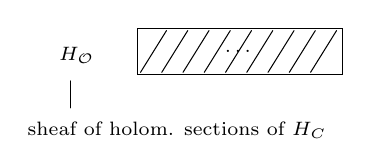
\begin{tikzpicture}[x=1mm,y=1mm,line cap=round,every node/.style={inner sep=0pt,font=\scriptsize}]
\node[anchor=base west] at (4,10.5) {$H_{\mathcal O}$};
\draw (14,8.7) rectangle (40,14.6);
\foreach \x in {14.4,17.1,19.8,22.5,25.2,27.9,30.6,33.3,36.0}
  \draw[line width=.37pt] (\x,9) -- ++(3.3,5.3);
\node at (27,11.65) {\sout{\ldots}};
\draw (5.5,7.9)--(5.5,4.5);
\node[anchor=base west] at (0,1) {\uwave{sheaf of holom. sections of \mbox{$H_{\mathbb C}$}}};
\end{tikzpicture}}\endgroup}
\end{GelfandAdjacentEvidence}
\begin{GelfandAdjacentEvidence}{GELFAND-P000456}{8}

\Unclear{GELFAND-P000456}{o-old-fragment}{The crossed-out entry may start with $H$ and a subscript.}
\end{GelfandAdjacentEvidence}
\begin{GelfandAdjacentEvidence}{GELFAND-P000456}{9}

\Incomplete{GELFAND-P000456}{o-cancelled}{The crossed-out entry inside the rectangle is illegible.}
\end{GelfandAdjacentEvidence}

\[
H_{\mathcal O}=H_{\mathbb Z}\otimes_{\mathbb Z}\mathcal O_S.
\]
There is a natural connection (Gauss–Manin)
\[
\nabla\colon H_{\mathcal O}\longrightarrow
\Omega_S^1\otimes_{\mathcal O_S}H_{\mathcal O}
\qquad\text{($\mathbb C$-lin. homom.)}
\]
$\Omega_S^1$ — holom. diff. forms of order $1$


\Needspace{7\baselineskip}
\begin{GelfandAdjacentEvidence}{GELFAND-P000457}{1}
